\documentclass[10pt,twocolumn]{article}
\usepackage[a4paper,margin=15mm]{geometry}
\usepackage{amsmath,amssymb}
\usepackage{amsthm}
\usepackage{graphicx}
\theoremstyle{definition}
\newtheorem{proposition}{Proposition}
\newtheorem{remark}{Remark}
\usepackage{booktabs,array,calc}
\usepackage[font=small,labelfont=bf]{caption}
\usepackage[colorlinks=true]{hyperref}
\providecommand{\tightlist}{\setlength{\itemsep}{0pt}\setlength{\parskip}{0pt}}
\renewcommand{\thesubsection}{\arabic{subsection}}
\makeatletter
\renewcommand{\@seccntformat}[1]{\csname the#1\endcsname.\quad}
\makeatother
\emergencystretch=3em
\allowdisplaybreaks
\setlength{\tabcolsep}{4pt}

\begin{document}
\title{Exact Audits of Worked Systems for the\\
Obstruction Calculus:\\
Counts, Witnesses, and Monitoring Design Rules}
\author{Amin Abaee\\[0.35em]
{\small Independent Researcher}\\[0.55em]
{\small\href{https://orcid.org/0000-0002-0019-1842}{ORCID: 0000-0002-0019-1842}}\\[0.3em]
{\small\href{mailto:amin\_abaee@ut.ac.ir}{amin\_abaee@ut.ac.ir}}}
\date{September 25, 2026}
\maketitle

\begin{abstract}
Viability certificates are useful in applications only insofar as their behaviour on concrete systems is understood precisely. This paper develops one exact audit framework --- integer and rational arithmetic throughout, every
count regenerated by script --- and applies it to a family of worked
systems that instantiate the mechanisms of the obstruction calculus
: a shared finite two-coordinate system with observation
structures (aggregation, policy-class restrictions, decentralized
observation, regime uncertainty), a review-timing grid for a
hidden-regime resource model, and a continuous two-floor production
benchmark. The audits yield the following. The review-timing identity on
the 93-cell grid is non-strict: viability at the deadline holds if and
only if \(T_{\mathrm{obs}} \le \tau^{*}(z_0) = z_0 - 1\), boundary included; the strict form against the real exit bound fails exactly on the boundary cells (against the floored count \(\sigma^{*}\), on one cell per row from \(z_0 = 2\)). On the four-state
monitoring target, 7 of the 15 partitions are adequate with two incomparable coarsest adequate two-cell partitions (minimal in the refinement order --- hence no single coarsest adequate design exists), and the two maximal common-action sets overlap. Four policy classes have kernel
sizes 24, 26, 25, and 28 of 36 belief pairs --- the classes form a two-by-two product of aggregation level and protocol --- with incomparable middle
cells. Decentralized unanimity over a
\(256\)-law space (\(64\) behaviorally distinct) sustains 12 of 36
pairs; a whole-law authority restriction collapses the kernel to zero,
and either agency's low vote forced against the target kills it. Under
frozen regimes no pair is lost (the corner pins its state); mode-blind
operation loses exactly the pairs containing the corner state
\((1,1)\). The biased certainty-equivalence law has
drift at least \(21/100\) on \([1,2]\); the bias-free law has drift
identically zero. The benchmark's critical aggregate is \(Y^{*} = 27/5\) (feasible,
margin \(0\)); at the audited obstructed aggregate \(Y = 6\) a
rational dual certificate prices the shortfall at margin \(3/50\). Static duality
holds at value \(-1/10\) on the two-floor instance with an \(\ell_1\)-normalized
Farkas pair, and a Helly-tight triple exhibits the sparse \(m{+}1\)-constraint witness. The complete result tables are carried here: the master table
of all 36 belief pairs against the five kernels, the sixteen sustaining
law pairs of the decentralized protocol (an exact \(4 \times 4\)
product), the 93-cell timing grid, the fifteen-partition census with
each fibre's common safe-action set, and the benchmark and drift tables,
with a five-figure set regenerated from the same scripts. Design rules
follow: review deadlines are boundary-inclusive; merged fibres call for
splits, not threshold tuning; aggregated indices support certainly-safe
reporting only; biased observation maps call for structural correction.
\end{abstract}

\textbf{Keywords:} viability kernels; obstruction certificates; exact
arithmetic; monitoring design; \mbox{decentralized observation}; certainty
equivalence

\subsection{Introduction}\label{introduction}

The obstruction calculus states sound sufficient conditions for
nonviability --- obstruction certificates --- mechanism by mechanism:
common-action failure (Sections \ref{master}--\ref{adequacy}),
review-timing failure (Section \ref{timing}), finite-time exit under
regime alternation (Section \ref{regimes}), and failure induced by
restricting the policy class or by a biased observation map
(Sections \ref{classes}, \ref{drift}) (Abaee, 2026b). Each mechanism is
accompanied in application by quantitative questions. How many belief
states does an observation structure destroy, and which ones? At which
review deadlines does the timing certificate fire, and does it fire at
the boundary? What exactly does a vote protocol cost, and which law in
the protocol's space sustains a given target? This paper answers such
questions exactly for a family of worked systems, under one audit frame
and one notation. The sharp thesis, made explicit by the master
theorem of Section~\ref{mtheorem}: obstructions arise from five
mechanisms --- common-action failure, memory/register coupling,
finite-time boundary exit, decentralized information loss, and joint
convex infeasibility --- and each admits a certificate with an explicit
semantic scope, a monotonicity status, and a robustness margin.

Three properties define the frame. First, all computations are carried
out in integer and rational arithmetic: no solver, no tolerance, no
simulation. Second, every discrete census in the family is finite --- the continuous objects reduce to exact rational calculations on rationally specified domains --- and every count is regenerated by a deterministic standard-library script, so any two executions agree. Third, each audited quantity is stated together with a
witness or a certificate --- an action sequence, a partition, a law
pair, a dual measure --- so the counts carry their own evidence. This paper carries the audit's complete result tables and its figure set:
the per-pair membership table behind the kernel counts, the sustaining
law pairs behind the decentralized count, the full timing grid, the full
partition census, and the benchmark and drift tables, every entry of
which is regenerated from the same scripts that verify the text.

The systems are drawn from the applied model of Abaee (2026a), in which
a two-coordinate resource stock is managed by acting one of two
instruments under incomplete observation. The family comprises: the
shared audit system with its observation structures (Sections
\ref{master}--\ref{decentralized} and \ref{adequacy}--\ref{regimes});
the hidden-regime review grid (Section
\ref{timing}); a continuous two-floor production benchmark (Section
\ref{benchmark}); and a multiple-floor line extending the Farkas
certificate to jointly binding constraints (Section \ref{floors}).

\subsection{Systems, conventions, and methods}\label{frame}

\emph{The shared audit system.} States are pairs
\(x = (z_1, z_2) \in \{0,1,2,3\}^{2}\); the safe set is
\(\mathcal{V} = \{z_1 \ge 1,\ z_2 \ge 1\}\) with the two coordinates as
floors. Instruments are \(u \in \{0, 1, 2\}\): \(u = j \in \{1,2\}\)
acts coordinate \(j\), which regenerates one unit up to the cap \(3\),
while the other coordinate loses one unit; \(u = 0\) executes no
instrument and both coordinates lose one. The transition is defined index-wise: the acted coordinate regenerates, \(F_j(z)_j = \min\{3,\ z_j + 1\}\), and the other declines, \(F_j(z)_{3-j} = \max\{0,\ z_{3-j} - 1\}\), for \(j \in \{1,2\}\); \(F_0(z)_i = \max\{0,\ z_i - 1\}\) for both coordinates \(i\) --- coordinates clip at zero, the cap is saturating --- and safety is evaluated after each transition. A coordinate-swapped misreading (the regenerated coordinate written first for both \(j\)) reproduces no audited count and is excluded by the verification script. Instrument \(0\) is never uniquely viable on the audited family: admitting \(u = 0\) as a third action leaves all four kernel counts unchanged (\(24, 26, 25, 28\); verified by the verification script, which also checks the structural premises --- \(F_0 \le F_1\) and \(F_0 \le F_2\) pointwise on the grid and the safe set an up-set, the one-step reason no fibre needs \(0\)). The corner \((1,1)\) is the
single state from which no instrument maintains both floors, so its
singleton is nonviable; the nine safe states generate
\(C(9,2) = 36\) two-element belief pairs, the audited population (28 of the pairs full-information-viable; column F of Table~\ref{tab:master}), at review horizon \(H = 12\) under the audited two-horizon verdict (the winning recursion at \(H\) and at \(H - 2\), which agree setwise on the audited universe and on the whole \(2^9\)-belief universe (stabilized from horizon \(2\) there, and from horizon \(1\) for the two non-alternation classes) --- \(W_{12} = W_{10}\) for each policy class, verified by the verification script --- so the verdict certifies a stabilized recursion; Abaee, 2026b, Theorem 1).

\emph{Observation structures.} An observation map
\(\mathrm{info}: x \mapsto c\) partitions a belief into fibres; a policy
acts per fibre on the read cell. The audited policy classes combine two
aggregation levels (full information; aggregation
\(c(x) = z_1 + z_2\)) with two protocols (free per-step choice; the
no-repeat protocol that forbids repeating the previous action. The
protocol's register is formalized as follows: one previous-action register
serves each review, shared by all fibres of the belief and not one per
branch; the policy fixes one action per fibre, the register then holds
some fibre's executed action, and the audited rule is pessimistic --- the
belief survives only if every admissible thread (each fibre's action
entering the register) leaves a winning continuation. Register values are
the two instruments, the initial register is unconstrained, and the survival condition quantifies over every
admissible thread, so the semantics is thread-independent by
construction (Proposition~\ref{prop:register} computes what
single-thread rules and per-branch registers give instead).

\emph{Exactness.} Counts are computed by backward recursion over fibre
partitions with exact state arithmetic; witnesses are extracted as step-one per-fibre action vectors along a winning branch; the certificate itself is the recursion invariant --- winning-set membership at every horizon level, quantified universally over adversarial successor states and register threads --- of which the archived step-one vector is the first level. The census of
Section \ref{adequacy} enumerates all \(15\) partitions of a four-state
target; partitions are ordered by refinement --- \(P\) is coarser than
\(P'\) when every fibre of \(P'\) lies in a fibre of \(P\) --- and
``coarsest adequate'' is relative to this order. The continuous objects of Section \ref{benchmark} are rationals.

\emph{Conventions.} On the hold class of the hidden-regime model, the
worst-case exit time is \(\tau^{*}(z_0) = z_0 - 1\) and the discrete
survival supremum (the largest admissible integer review count) is
\(\sigma^{*}(z_0) = \lfloor z_0 - 1 \rfloor = \lfloor \tau^{*}(z_0)
\rfloor\), with level sets \(\{z_0 \ge 1 + k\}\); for an integer deadline
the inclusive criterion \(T_{\mathrm{obs}} \le \tau^{*}(z_0)\) coincides
with \(T_{\mathrm{obs}} \le \sigma^{*}(z_0)\), while the strict form
against the floored count is stricter than against the real exit time off
integer \(\tau^{*}\). Two
certainty-equivalence laws are audited: an uncorrected law whose index
leads the state by one step, \(s \mapsto s + 0.1\), and a corrected law
with the lead removed; both are read through the index \(g(s) = s^{2}\).

\emph{Figures and tables.} Every figure and every tabulated entry in
this paper is produced by a generation script that first recomputes the
quantity from the primitives above, in exact rational arithmetic, and
asserts it before drawing or printing; the master verification script of
Section \ref{methods} chains both scripts and re-derives the tabulated
entries independently.

\subsection{A master monotonicity theorem}\label{mtheorem}

The audited family is an instance of one abstract object, and its
kernel comparisons are instances of one theorem. An \emph{audited
tuple} is
\(\Theta = (X, \mathcal{V}, A, F, \mathrm{info}, \Pi, m)\): a finite
state set \(X\) with safe set \(\mathcal{V}\), action set \(A\),
transition \(F\), observation map, admissible policy class \(\Pi\)
(per-cell action rules), and register convention \(m\) (shared, per-branch,
or none); viability is the horizon-stabilized recursion of
Section~\ref{frame}.

\begin{proposition}[master monotonicity]\label{prop:master}
Fix the audited tuple. Kernel membership is monotone in each of the
three enlargements, setwise: (i) \emph{policies}: if
\(\Pi \subseteq \Pi'\) then
\(\mathcal{W}_{\Pi} \subseteq \mathcal{W}_{\Pi'}\) --- restriction is
antitone (Proposition~\ref{prop:lattice}); (ii) \emph{observations}:
if \(\mathrm{info}'\) is finer than \(\mathrm{info}\) (every fibre of
\(\mathrm{info}\) is a union of fibres of \(\mathrm{info}'\)) then
\(\mathcal{W}_{\mathrm{info}} \subseteq
\mathcal{W}_{\mathrm{info}'}\); (iii) \emph{memory}: a per-branch
register dominates the shared register --- every shared-register policy
is a per-branch policy, so the per-branch kernel contains the shared
one. Finer observation maps and larger memories can only enlarge the
kernel; all three statements are proved by the same induction on the
horizon: each enlargement enlarges the admissible action sets at every
cell and horizon level, so a winning continuation transfers upward.
\end{proposition}

\begin{proof}
Induction on \(h\). For \(h = 0\) the kernels coincide
(\(\mathcal{V}\) is fixed). Step: a belief winning at \(h\) under the
restricted tuple uses, at each cell, an action admissible and winning
there; the same choice is admissible under the enlarged tuple (the
action set at each cell only grows: more policies choose more actions,
finer cells shrink the quantifier over merged branches, a branch-local
register relaxes the no-repeat constraint on the other branch), and the
continuation is winning at \(h-1\) by the inductive hypothesis. The
finite population makes the induction an exact certificate: checks
P16--P18 verify the containments setwise on all \(36\) pairs.
\end{proof}

The audited counts are the theorem's rows: \(24 \le 26\) and
\(25 \le 28\) (observation axis, free protocol), \(24 \le 25\) and
\(26 \le 28\) (protocol axis at fixed aggregation), and the
per-branch-register kernels \((26, 26, 27)\) dominate the shared ones
\((24, 26, 25)\) (memory axis; Proposition~\ref{prop:register}).
\begin{proposition}[stationary policies]\label{prop:stationary}
Enumerate all deterministic stationary policies --- one action per cell,
fixed in time: \(2^{9} = 512\) at full information (nine singleton
cells), \(2^{5} = 32\) at aggregation (sums two to six). At full
information the union of the stationary policies' safe-pair sets is
exactly the kernel: memoryless sufficiency holds on the instance, and
the \(28\)-pair kernel admits an independent constructive description.
At aggregation the union is \emph{empty} --- no stationary policy
sustains any of the \(36\) pairs: the merged index is read against
states that demand conflicting actions across visits, and every
aggregate-viable pair relies on actions scheduled against time. The
\(26\)-pair aggregate kernel is therefore entirely a time-varying-policy
phenomenon --- the register-coupling mechanism in another guise, with
the review clock in the register's place (checks P17--P18; the fixpoint
computation of each class's horizon family independently reproduces all
four kernels).
\end{proposition}

\begin{proof}
Both counts are exhaustive enumerations with exact forward simulation
under each fixed policy (check P17), cross-validated against the
backward recursion by the horizon fixpoint (check P18).
\end{proof}

Strictness is instance-specific: the strict differences are exactly the
register-blocked pairs \(\{(1,2),(3,1)\}\) and \(\{(1,3),(2,1)\}\) on
the protocol axis, the single pair \(\{(1,3),(3,1)\}\) on the
observation axis, with the alternation-forced pair \(\{(1,2),(2,1)\}\)
outside both middle kernels; the incomparability of the
middle cells is a shared-register phenomenon, and the decentralized
kernel sits outside the chain because unanimity restricts \emph{who}
acts, not what the acting policy may do --- an orthogonal axis the
theorem prices separately (Section~\ref{decentralized}).

\subsection{The master table}\label{master}

Table \ref{tab:master} is the audit's master table: all 36 belief pairs
against the five kernels --- the four policy classes of Section
\ref{classes} (institutional: one shared compliance register per
review; aggregate: one pooled index per branch; full-information codex:
pooled registers across branches; full-information: unrestricted state
observation) and the decentralized kernel of Section
\ref{decentralized}. Rows are grouped by the pair's lexicographically
smaller state, written \(z_1 z_2\).

\begin{table*}[t]
\centering
\footnotesize
\caption{The master table: membership of all 36 belief pairs in the five
audited kernels. I = institutional (aggregation, no-repeat); A =
aggregate; C = full-information codex; F = full information; D =
decentralized unanimity. A dot marks a non-member; every entry is
regenerated by script.}
\label{tab:master}
\begin{tabular}{@{}l cccc c@{\hspace{12pt}}l cccc c@{}}
\toprule
Pair & I & A & C & F & D & Pair & I & A & C & F & D\\
\midrule
$12|21$ & $\cdot$ & $\cdot$ & $\cdot$ & F & D &
$22|31$ & I & A & C & F & D\\
$12|31$ & $\cdot$ & A & $\cdot$ & F & $\cdot$ &
$22|23$ & I & A & C & F & $\cdot$\\
$12|23$ & I & A & C & F & D &
$22|33$ & I & A & C & F & D\\
$12|33$ & I & A & C & F & $\cdot$ &
$22|32$ & I & A & C & F & $\cdot$\\
$12|22$ & I & A & C & F & $\cdot$ &
$23|31$ & I & A & C & F & $\cdot$\\
$12|32$ & I & A & C & F & D &
$23|33$ & I & A & C & F & $\cdot$\\
$12|13$ & I & A & C & F & $\cdot$ &
$23|32$ & I & A & C & F & D\\
$13|21$ & $\cdot$ & A & $\cdot$ & F & $\cdot$ &
$31|33$ & I & A & C & F & D\\
$13|31$ & $\cdot$ & $\cdot$ & C & F & D &
$31|32$ & I & A & C & F & $\cdot$\\
$13|23$ & I & A & C & F & $\cdot$ &
$32|33$ & I & A & C & F & $\cdot$\\
$13|33$ & I & A & C & F & D &
$11|12$ & $\cdot$ & $\cdot$ & $\cdot$ & $\cdot$ & $\cdot$\\
$13|22$ & I & A & C & F & D &
$11|21$ & $\cdot$ & $\cdot$ & $\cdot$ & $\cdot$ & $\cdot$\\
$13|32$ & I & A & C & F & $\cdot$ &
$11|31$ & $\cdot$ & $\cdot$ & $\cdot$ & $\cdot$ & $\cdot$\\
$21|31$ & I & A & C & F & $\cdot$ &
$11|23$ & $\cdot$ & $\cdot$ & $\cdot$ & $\cdot$ & $\cdot$\\
$21|23$ & I & A & C & F & D &
$11|33$ & $\cdot$ & $\cdot$ & $\cdot$ & $\cdot$ & $\cdot$\\
$21|33$ & I & A & C & F & $\cdot$ &
$11|22$ & $\cdot$ & $\cdot$ & $\cdot$ & $\cdot$ & $\cdot$\\
$21|22$ & I & A & C & F & $\cdot$ &
$11|32$ & $\cdot$ & $\cdot$ & $\cdot$ & $\cdot$ & $\cdot$\\
$21|32$ & I & A & C & F & D &
$11|13$ & $\cdot$ & $\cdot$ & $\cdot$ & $\cdot$ & $\cdot$\\
\bottomrule
\end{tabular}
\end{table*}

The column counts are the audited kernel sizes
\(|\mathcal{W}_{\mathrm{inst}}| = 24\),
\(|\mathcal{W}_{\mathrm{agg}}| = 26\),
\(|\mathcal{W}_{\mathrm{full\text{-}codex}}| = 25\),
\(|\mathcal{W}_{\mathrm{full}}| = 28\), and
\(|\mathcal{W}_{\mathrm{dec}}| = 12\). Figure \ref{fig:kernels} displays
the four policy-class kernels, whose middle cells are incomparable. Two set-level facts are recorded exactly. The meet of the
two middle kernels equals the institutional kernel setwise. At class
level the join is the full-information class; at kernel level the union
of the two middle kernels falls one pair short of the full kernel:
exactly the pair \(\{(1,2),(2,1)\}\) lies in neither middle kernel. The
pair is the alternation-forced pair: under full information each branch
survives by its own strict alternation --- \((1,2)\) under \(1, 2, 1,
\dots\) and \((2,1)\) under \(2, 1, 2, \dots\) --- which the
idealized per-state policy can carry on both branches; aggregation cannot
see either requirement (one fibre, no common action), and the no-repeat
protocol, whose single previous-action register must serve both branches,
forbids the second branch's required next action once the first branch's
choice occupies the register. The full kernel is exactly the
\(C(8,2) = 28\) pairs avoiding the corner \((1,1)\): the corner's
singleton nonviability accounts for every remaining pair-level loss at
full information, as the eight \(11|\cdot\) rows of Table
\ref{tab:master} show.

\begin{figure}[t]
\centering
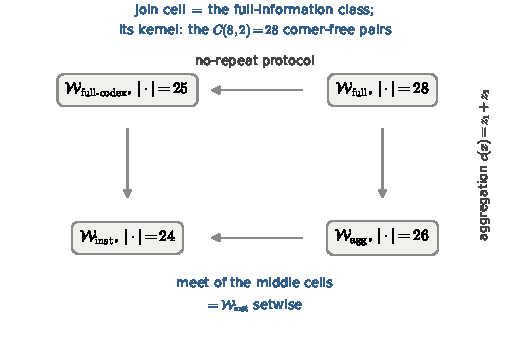
\includegraphics[width=0.94\linewidth]{figs_ws4/fig_kernels.pdf}
\caption{The four policy classes form a two-by-two product of aggregation
level and protocol; the audited kernel sizes are \(24, 26, 25, 28\) of
36. The meet of the middle kernels is the institutional kernel setwise;
the class join is the full-information class, whose kernel is the 28
corner-free pairs, one pair beyond the middle-kernel union.}
\label{fig:kernels}
\end{figure}

\subsection{Policy classes}\label{classes}

The four audited classes combine full information and aggregation with
free and no-repeat protocols. Their kernels among the 36 pairs have
sizes:
\begin{gather*}
|\mathcal{W}_{\mathrm{inst}}| = 24,\quad
|\mathcal{W}_{\mathrm{agg}}| = 26,\\
|\mathcal{W}_{\mathrm{full\text{-}codex}}| = 25,\quad
|\mathcal{W}_{\mathrm{full}}| = 28 .
\end{gather*}
The four classes form a two-by-two product of aggregation level and
protocol; their kernels have incomparable middle cells:
the aggregate kernel contains pairs outside the full-information codex
kernel (for instance \(\{(1,2),(3,1)\}\) and \(\{(1,3),(2,1)\}\)), and
the codex kernel contains pairs outside the aggregate (for instance
\(\{(1,3),(3,1)\}\)). Within each observation column the free protocol's
kernel contains the no-repeat protocol's (both inclusions strict); across
columns neither middle kernel contains the other. The precise
meet-and-join reading is the one recorded in Section \ref{master}. Two
per-pair readings illustrate the columns of Table \ref{tab:master}. The
pair \(\{(1,2),(3,1)\}\) is aggregate-viable but not codex-viable: the
free protocol admits it under both observation structures, while the
no-repeat protocol excludes it under both --- at the second review the
thread that records the \((3,1)\)-branch's instrument \(2\) forbids the
forced instrument \(2\) of the successor branch \((2,1)\), the same
shared-register collision that excludes the alternation-forced pair. The pair \(\{(1,3),(3,1)\}\) is
codex-viable but not aggregate-viable: the two branches share the fibre
\(c = 4\), and no single per-fibre instrument serves both, while
full information separates them. Three structural facts behind the table
admit short proofs.

\begin{proposition}[full information decomposes branchwise]\label{prop:decomp}
At full information under the free protocol, a two-state belief is
viable if and only if each of its singletons is viable; the kernel is
exactly the \(C(8,2) = 28\) corner-free pairs.
\end{proposition}

\begin{proof}
Full-information fibres are singletons, so a belief's step-one action
sets are the product of its branches': a choice is admissible exactly
when each branch's part is, and the recursion decomposes --- a belief is
viable exactly when both branches are. For the singletons: the corner
\((1,1)\) is nonviable because each instrument drops a coordinate to
zero in one step (\(u = 1\) forces \(z_2 = 0\), \(u = 2\) forces
\(z_1 = 0\), \(u = 0\) forces both); every other singleton is viable
--- the memoryless policy that plays instrument \(1\) exactly at
\(z_1 = 1\) and instrument \(2\) otherwise is safe forever: at
\(z_1 = 1\) the exclusion of the corner gives \(z_2 \ge 2\), so
\(u = 1\) restores \(z_1 = 2\) with \(z_2 \ge 1\); at
\(z_1 \ge 2\), \(u = 2\) keeps \(z_1 \ge 1\) and regenerates
\(z_2\).
\end{proof}

\begin{proposition}[class lattice]\label{prop:lattice}
Kernel membership is antitone in the policy class: restricting the class
can only lose viable beliefs. Hence
\(\mathcal{W}_{\mathrm{inst}} \subseteq \mathcal{W}_{\mathrm{agg}},
\mathcal{W}_{\mathrm{full\text{-}codex}} \subseteq
\mathcal{W}_{\mathrm{full}}\); on the audited 36-pair population the
two middle inclusions are strict, the meet
\(\mathcal{W}_{\mathrm{agg}} \cap
\mathcal{W}_{\mathrm{full\text{-}codex}}\) equals the institutional
kernel setwise, and exactly one pair --- the alternation-forced pair
\(\{(1,2),(2,1)\}\) --- lies in the full kernel outside the middle
union.
\end{proposition}

\begin{proof}
Antitonicity --- order-reversal between class inclusion and kernel inclusion --- is immediate: a policy admissible for a restricted class is
admissible for any enlargements, so viability transfers upward. The
setwise facts are finite statements about a 36-element population; they
are proved by exhaustive certification --- the master table's
\(36 \times 5\) membership marks are recomputed row-by-row by the paper's verification script (checks M2 and M5), which is a complete
proof for a finite family.
\end{proof}

\begin{proposition}[register-semantics invariance]\label{prop:register}
Endow the no-repeat protocol with the pessimistic shared-register
semantics: the policy fixes one action per fibre, the register then holds
some fibre's executed action, and the belief survives only if every
admissible thread leaves a winning continuation. Because the survival condition
quantifies universally over threads, the
pessimistic kernels depend on no thread choice: the audited counts
\(24, 26, 25, 28\) are thread-independent by construction. Two further
readings are computed for the record. A single-thread rule (one fixed
fibre's action entering the register) is order-sensitive: with the
first, or the last, fibre in sorted order the counts are
\(25, 26, 26, 28\) --- neither fixed rule yields the audited
institutional and codex counts --- so the well-defined semantics is the
pessimistic one. The optimistic semantics (some thread) is strictly
larger (codex \(27\)) and is not the audited reading. If instead each
branch carries its own register --- one compliance record per unit,
threaded forward along the branch --- the protocol cost collapses: the
institutional kernel equals the aggregate kernel setwise (\(26 = 26\)),
and the codex kernel becomes \(27\), regaining the alternation-forced
pair and losing exactly \(\{(1,3),(3,1)\}\) relative to full
information, with the aggregate kernel contained in it. The
incomparability of the middle cells is therefore a shared-register
phenomenon; the shared register is the audited institutional object ---
one compliance register per review across the units managed under the
protocol.
\end{proposition}

\begin{proof}
Every clause is a finite statement, computed from the shared primitives
of Section \ref{frame} and asserted by the verification script: the
pessimistic counts (M2b), the optimistic containment (M2c), both
single-thread orders, and the per-branch kernels with the
\(\{(1,3),(3,1)\}\) loss (checks P9 and P10).
\end{proof}

\subsection{Decentralized observation}\label{decentralized}

Two agencies each observe one coordinate and vote; an instrument
executes only on agreement. Each agency's vote is a map from its
coordinate's four values to the two instruments, so the law space has
\(2^{4} \times 2^{4} = 256\) law pairs. Unanimity sustains 12 of the
36 pairs (column D of Table \ref{tab:master}), and exactly 16
coordinated-viable pairs are lost. The loss instance
\(\{(1,2),(3,1)\}\) is representative: each branch is individually
sustainable, and no law pair sustains the belief. For the audited belief
\(\{(1,2),(2,1)\}\), exactly 16 of the 256 law pairs sustain it; the
count coincides numerically with the 16 lost pairs, and no identity is
implied. The authority restriction is exact:

\begin{proposition}[authority restriction]\label{prop:authority}
Fixing agency 2's vote at \(z_2 = 1\) to instrument \(1\) sustains no
law pair for the belief \(\{(1,2),(2,1)\}\): branch \((2,1)\) exits
at its first step under every such law pair. Fixing agency 1's vote at
\(z_1 = 1\) to instrument \(1\) leaves exactly the \(16\) sustaining
law pairs of Table \ref{tab:laws}, and either whole-law
restriction (one agency's vote fixed to a single instrument at every
level) collapses the decentralized kernel to zero.
\end{proposition}

\begin{proof}
On branch \((2,1)\) at the first step: \(z_2 = 1\) must not
decline, so agreement on instrument \(2\) is required; agency 2's
fixed vote at \(z_2 = 1\) is \(1\), so agreement can hold only on
instrument \(1\), which drives \(z_2\) to zero, and disagreement
executes \(u = 0\), which does the same --- the branch exits at step
one under every admissible law pair. With agency 1's vote at \(z_1 = 1\) fixed to \(1\), the
sustaining pairs are exactly those with agency 1 forced to \(1\) at
\(z_1 = 1\) and \(2\) at \(z_1 = 2\) and agency 2 forced to \(2\)
at \(z_2 = 1\) and \(1\) at \(z_2 = 2\) (each forcing is a
one-step safety requirement: the low coordinate must regenerate), and
the free votes at \(\{0, 3\}\) never bind --- the \(4 \times 4\)
product of Table \ref{tab:laws}. A whole-law restriction
fixes one agency's vote everywhere; the other agency's coordinate then
cannot regenerate at the low states where the fixed vote disagrees, and
the kernel collapses (verified exhaustively over all \(256\) law pairs, the whole-law
kernels \(0\) in all four cases; check P12 of the verification script).
\end{proof}

\begin{table}[t]
\centering
\footnotesize
\caption{The 16 law pairs sustaining the audited belief
\(\{(1,2),(2,1)\}\) factor exactly: agency 1's vote is forced to
\(1\) at \(z_1 = 1\) and \(2\) at \(z_1 = 2\), free at
\(z_1 \in \{0, 3\}\); agency 2's vote is forced to \(2\) at
\(z_2 = 1\) and \(1\) at \(z_2 = 2\), free at
\(z_2 \in \{0, 3\}\). Every combination sustains --- a complete
\(4 \times 4\) product (votes listed as
\((l(z{=}0), l(z{=}1), l(z{=}2), l(z{=}3))\));
agency 1's votes are the row labels, agency 2's the column labels.}
\label{tab:laws}
\begin{tabular}{@{}l cccc@{}}
\toprule
 & \multicolumn{4}{c}{agency 2}\\
\cmidrule(l){2-5}
agency 1 & 1211 & 1212 & 2211 & 2212\\
\midrule
1121 & \checkmark & \checkmark & \checkmark & \checkmark\\
1122 & \checkmark & \checkmark & \checkmark & \checkmark\\
2121 & \checkmark & \checkmark & \checkmark & \checkmark\\
2122 & \checkmark & \checkmark & \checkmark & \checkmark\\
\bottomrule
\end{tabular}
\end{table}

The law space itself is counted before quotienting: a \(z = 0\) vote is
consultable only on a trajectory that has already left the safe set, so
the audited kernel is invariant under the \(z{=}0\)-vote quotient ---
the effective law space is \(2^{3} \times 2^{3} = 64\) behaviorally
distinct law pairs, and the \(16\) sustaining law pairs of Table
\ref{tab:laws} comprise \(4\) distinct behavioral laws times the \(4\)
never-consulted \(z{=}0\) votes. The sustaining set has an
exact product structure (Table
\ref{tab:laws}): on the trajectory alternating between the branches,
agency 1 is read only at \(z_1 \in \{1, 2\}\) and must vote \(1\) then
\(2\); agency 2 is read only at \(z_2 \in \{2, 1\}\) and must vote
\(1\) then \(2\); the votes at the unreachable coordinates
\(z \in \{0, 3\}\) are free, giving \(2^{2} \times 2^{2} = 16\). The
restricted kernels are exact. Fixing either agency's low vote to the
regenerating instrument (agency 1 to \(1\) at \(z_1 = 1\), agency 2 to
\(2\) at \(z_2 = 1\)) leaves the decentralized kernel untouched at
\(12\) --- the constraint does not bind. Fixing either agency's low
vote against it (agency 2 to \(1\) at \(z_2 = 1\), agency 1 to \(2\)
at \(z_1 = 1\)) shrinks the kernel to four beliefs ---
\(\{(2,3),(3,2)\}\), \(\{(2,2),(3,3)\}\), \(\{(1,3),(3,3)\}\),
\(\{(1,3),(2,2)\}\), up to the symmetry below --- and kills the
audited target; a whole-law restriction collapses the kernel to \(0\)
in all four cases. The model's swap symmetry (coordinates and instruments
together) interchanges the agencies and maps the audited target to
itself, so no agency is privileged: what carries the target is the
direction of each forced vote --- each branch's low coordinate must be
allowed to regenerate --- not the agency holding it. Two modelling choices are declared. The deadlock transition
\(u = 0\) executes no instrument and both coordinates lose one; and
each agency votes on its own coordinate's current value: the audited
protocol is memoryless and decentralized --- no agency observes the
belief, the other agency's observation, or anything like common
knowledge. The count has a theorem behind it:

\begin{proposition}[the decentralized kernel factors statewise]
\label{prop:req}
Unanimity executes statewise: the executed instrument at a state depends
only on the two votes at that state's coordinates, and safety is
evaluated per state. Hence a belief is sustained if and only if its
branches share a common sustaining law pair,
\(\bigcap_{x \in B} S(x) \neq \emptyset\), where \(S(x)\) is the set
of law pairs sustaining the singleton \(\{x\}\); on the audited
population the factored criterion reproduces the joint kernel exactly
(the \(12\) sustained beliefs of the master table), and the \(16\)
sustaining law pairs of the audited belief
(Table~\ref{tab:laws}) are invariant under the model's coordinate-swap
symmetry. The obstruction is legible branchwise: a belief is lost
exactly when its branches' sustaining sets do not intersect --- as for
the representative loss \(\{(1,2),(3,1)\}\), each branch individually
sustainable, no law pair sustaining both.
\end{proposition}

\begin{proof}
The belief trajectory under a law pair is the union of the branch
trajectories (statewise execution, statewise safety), so it stays in
\(\mathcal{V}\) if and only if every branch trajectory does --- which is
the displayed intersection. Both computations (the factored singleton
intersection and the joint \(256\)-pair enumeration) are run on all
\(36\) beliefs and agree setwise (check P20). The symmetry is the swap
map of this section's closing remark applied to the product structure.
\end{proof}

\subsection{Review timing on the hidden-regime grid}\label{timing}

The hidden-regime resource model: a single stock held at level
\(z_0 \ge 1\) above the floor; each review period the unobserved
adversarial regime realizes one unit of decline and there is no
regeneration (the hold class), so the stock tracks \(z(t) = z_0 - t\)
and remains safe exactly while \(z(t) \ge 1\). The model is audited on
the grid \(z_0 \in \{1.0, 1.1, \dots, 4.0\}\) and
\(T_{\mathrm{obs}} \in \{1, 2, 3\}\), 93 cells. Viability at the
deadline holds if and only if
\(T_{\mathrm{obs}} \le \tau^{*}(z_0) = z_0 - 1\), with zero
mismatches across the grid. The identity is boundary-inclusive: the
viable cells number \(33\), and the strict form \(T_{\mathrm{obs}} <
\tau^{*}(z_0)\) fails exactly on the boundary cells \((2,1)\),
\((3,2)\), and \((4,3)\) --- those with \(z_0 = 1 +
T_{\mathrm{obs}}\); against the floored count \(\sigma^{*}\) the
strict form fails on one cell per row \(z_0 \ge 2\) --- \(21\) cells,
the boundary cells included --- which is why the
inclusive predicate is the audited identity.
Table \ref{tab:timing} carries the full grid and Figure
\ref{fig:timing} displays it. The practical form of the rule: a review
must land no later than the worst-case exit time, and a deadline exactly at the worst-case exit is admissible under the audited endpoint convention (closed safe set; safety evaluated at the deadline review); no open-set or alternative-exit-convention claim is made. The audited identity is in fact the
restriction of a general law:

\begin{proposition}[review timing, general form]\label{prop:timing}
On the hold class of the hidden-regime model, for every initial level
\(z_0 \ge 1\) and every integer deadline \(T \ge 0\), the cell
\((z_0, T)\) is deadline-viable if and only if \(T \le z_0 - 1\).
Accordingly \(\sigma^{*}(z_0) = \lfloor z_0 - 1 \rfloor\) with
superlevel sets \(\{z_0 \ge 1 + k\}\), \(k \in
\mathbb{Z}_{\ge 0}\), and the audited 93-cell grid is the restriction
to \(z_0 \in \{1.0, \dots, 4.0\}\), \(T \in \{1, 2, 3\}\).
\end{proposition}

\begin{proof}
Under every admissible hold-class control the adversarial regime realizes
the declining branch at each step, so the worst stock declines at unit
rate and remains safe exactly through time \(z_0 - 1\) --- the last
safe review, the first violation occurring at \(z_0\):
deadline-viability forces \(T \le z_0 - 1\). Conversely
the hold policy tracks the decline path \(z(t) = z_0 - t\) branchwise,
which stays admissible exactly on \([0,\, z_0 - 1]\) and terminates at
the floor, which is safe because the safe set is closed; hence
\(T \le z_0 - 1\) is viable, boundary included. The set identity
\(\{T : T \le z_0 - 1\} = \{T : T \le \sigma^{*}(z_0)\}\)
(integer \(T\), all \(z_0\)) --- equivalently \(\{T < z_0 - 1\} =
\{T \le \sigma^{*}(z_0)\}\) off the integers, with the boundary
failure at integer \(z_0 - 1\) --- gives the displayed supremum.
\end{proof}

\begin{proposition}[hitting times on regime graphs]\label{prop:regime}
Let the adversary choose a regime path \(r_1 r_2 \dots\) through a
finite regime graph with per-step damages \(d_r \ge 0\), subject to
the graph's adjacency constraint. The worst cumulative damage by time
\(t\) is the max-plus recursion
\(D_t = \max_{\text{paths}} \sum_{s \le t} d_{r_s}\), and the cell
\((z_0, T)\) is deadline-viable if and only if \(D_T \le z_0 - 1\)
(the audited endpoint convention). Two exact instances: with free
switching the adversary plays the worst regime every step, \(D_t = t
\cdot \max_r d_r\), recovering Proposition~\ref{prop:timing} on the
audited grid; with two regimes of damages \(1\) and \(1/2\) forced to
alternate, the worst damage is \(D_{2k} = 3k/2\) and \(D_{2k+1} = 3k/2
+ 1\), and the re-audited \(93\)-cell grid has exactly \(43\) viable
cells (\(21, 16, 6\) at \(T = 1, 2, 3\)), zero mismatches between the
closed form and path enumeration. The max-plus dynamic program equals
path enumeration exactly on a three-regime graph with a forbidden
self-loop (all horizons to six).
\end{proposition}

\begin{proof}
Deadline-viability is safety of the worst adversarial path to the
deadline, which is the max-plus evaluation of the damage sum; free
switching decouples the steps, giving \(t \cdot \max_r d_r = t\) on
the audited damages and hence the audited identity. Under alternation
the two interleavings give \(D_{2k} = k(1 + \tfrac12) = 3k/2\) and
\(D_{2k+1} = (k+1) + \tfrac{k}{2}\); the grid recomputation enumerates
both interleavings per cell (check P21). The DP evaluation over
(last regime, step) is exact rational arithmetic and is asserted equal
to explicit path enumeration.
\end{proof}

\begin{table}[t]
\centering
\footnotesize
\caption{The timing grid, printed in full (\(93\) cells): viability at the deadline against \(\sigma^{*}(z_0) = \lfloor
\tau^{*}(z_0) \rfloor\) (the deadline count; the identity columns use
the inclusive predicate, on which the floored and real-valued forms
coincide). The checkmark of column
\(T_{\mathrm{obs}}\) means the cell is viable; the identity
column ``id.'' is the predicate
\(T_{\mathrm{obs}} \le \sigma^{*}(z_0)\) and column ``cell'' the audited
viability; the two agree on all \(93\) cells (zero mismatches; \(33\)
viable cells). The circled cell of Figure \ref{fig:timing} is
\((2.0, 1)\): viable, on the boundary; the strict form disagrees
exactly on the boundary cells \((2,1)\), \((3,2)\), \((4,3)\).}
\label{tab:timing}
\begin{tabular}{@{}l c c cc c cc c@{}}
\toprule
 & & \multicolumn{2}{c}{$T_{\mathrm{obs}} = 1$} &
\multicolumn{2}{c}{$T_{\mathrm{obs}} = 2$} &
\multicolumn{2}{c}{$T_{\mathrm{obs}} = 3$}\\
\cmidrule(lr){3-4}\cmidrule(lr){5-6}\cmidrule(lr){7-8}
$z_0$ & $\sigma^{*}$ & id. & cell & id. & cell & id. & cell\\
\midrule
1.0 & 0 & $\cdot$ & $\cdot$ & $\cdot$ & $\cdot$ & $\cdot$ & $\cdot$\\
1.1 & 0 & $\cdot$ & $\cdot$ & $\cdot$ & $\cdot$ & $\cdot$ & $\cdot$\\
1.2 & 0 & $\cdot$ & $\cdot$ & $\cdot$ & $\cdot$ & $\cdot$ & $\cdot$\\
1.3 & 0 & $\cdot$ & $\cdot$ & $\cdot$ & $\cdot$ & $\cdot$ & $\cdot$\\
1.4 & 0 & $\cdot$ & $\cdot$ & $\cdot$ & $\cdot$ & $\cdot$ & $\cdot$\\
1.5 & 0 & $\cdot$ & $\cdot$ & $\cdot$ & $\cdot$ & $\cdot$ & $\cdot$\\
1.6 & 0 & $\cdot$ & $\cdot$ & $\cdot$ & $\cdot$ & $\cdot$ & $\cdot$\\
1.7 & 0 & $\cdot$ & $\cdot$ & $\cdot$ & $\cdot$ & $\cdot$ & $\cdot$\\
1.8 & 0 & $\cdot$ & $\cdot$ & $\cdot$ & $\cdot$ & $\cdot$ & $\cdot$\\
1.9 & 0 & $\cdot$ & $\cdot$ & $\cdot$ & $\cdot$ & $\cdot$ & $\cdot$\\
2.0 & 1 & \checkmark & \checkmark & $\cdot$ & $\cdot$ & $\cdot$ & $\cdot$\\
2.1 & 1 & \checkmark & \checkmark & $\cdot$ & $\cdot$ & $\cdot$ & $\cdot$\\
2.2 & 1 & \checkmark & \checkmark & $\cdot$ & $\cdot$ & $\cdot$ & $\cdot$\\
2.3 & 1 & \checkmark & \checkmark & $\cdot$ & $\cdot$ & $\cdot$ & $\cdot$\\
2.4 & 1 & \checkmark & \checkmark & $\cdot$ & $\cdot$ & $\cdot$ & $\cdot$\\
2.5 & 1 & \checkmark & \checkmark & $\cdot$ & $\cdot$ & $\cdot$ & $\cdot$\\
\midrule
2.6 & 1 & \checkmark & $\cdot$ & $\cdot$\\
2.7 & 1 & \checkmark & $\cdot$ & $\cdot$\\
2.8 & 1 & \checkmark & $\cdot$ & $\cdot$\\
2.9 & 1 & \checkmark & $\cdot$ & $\cdot$\\
3.0 & 2 & \checkmark & \checkmark & $\cdot$\\
3.1 & 2 & \checkmark & \checkmark & $\cdot$\\
3.2 & 2 & \checkmark & \checkmark & $\cdot$\\
3.3 & 2 & \checkmark & \checkmark & $\cdot$\\
3.4 & 2 & \checkmark & \checkmark & $\cdot$\\
3.5 & 2 & \checkmark & \checkmark & $\cdot$\\
3.6 & 2 & \checkmark & \checkmark & $\cdot$\\
3.7 & 2 & \checkmark & \checkmark & $\cdot$\\
3.8 & 2 & \checkmark & \checkmark & $\cdot$\\
3.9 & 2 & \checkmark & \checkmark & $\cdot$\\
4.0 & 3 & \checkmark & \checkmark & \checkmark\\
\bottomrule
\end{tabular}
\end{table}

\begin{figure}[t]
\centering
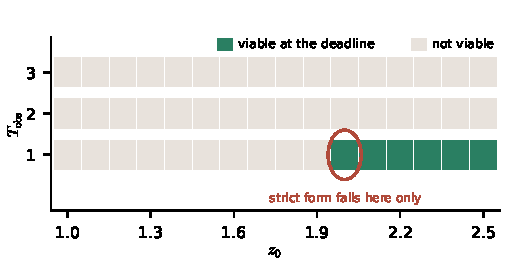
\includegraphics[width=0.96\linewidth]{figs_ws4/fig_timing.pdf}
\caption{The timing grid. Cells viable at the deadline (green) satisfy \(T_{\mathrm{obs}} \le \tau^{*}(z_0)\); the identity is
boundary-inclusive, and the strict form \(T_{\mathrm{obs}} <
\tau^{*}(z_0)\) fails at exactly one cell,
\((z_0, T_{\mathrm{obs}}) = (2.0, 1)\) (circled); against the floored count \(\sigma^{*}(z_0) = \lfloor z_0 - 1 \rfloor\) the strict form fails on all six viable cells, which is why the inclusive predicate is the audited identity.}
\label{fig:timing}
\end{figure}

\subsection{Monitoring adequacy}\label{adequacy}

Let \(R(x)\) denote the safe actions of state \(x\): those keeping
\(x\) in \(\mathcal{V}\) for one step. On the audited target,
\(R((1,2)) = \{1\}\), \(R((2,1)) = \{2\}\), \(R((2,2)) = \{1,2\}\), and
\(R((3,1)) = \{2\}\). A partition of a target belief is \emph{adequate}
when every fibre has a nonempty common safe-action set. On the
four-state target \(\{(1,2), (2,1), (2,2), (3,1)\}\), 7 of the 15
partitions are adequate, and two minimal adequate partitions with two
cells exist. Table \ref{tab:census} carries the complete census with
each fibre's common safe-action set; Figure \ref{fig:census} displays
it.

\begin{table}[t]
\centering
\footnotesize
\caption{The fifteen-partition census on the target
\(\{(1,2), (2,1), (2,2), (3,1)\}\) (states written \(z_1 z_2\); fibres
separated by ``;''). A partition is adequate when every fibre's common
safe-action set (brackets; \(\cdot\) = empty) is nonempty. Seven
partitions are adequate; the minimal adequate two-cell partitions are
rows 6 and 7.}
\label{tab:census}
\begin{tabular}{@{}l l l@{}}
\toprule
Partition & Adequate & Common safe actions\\
\midrule
$12|21|22|31$ & no & $[\cdot]$\\
$12|21|31$ ; $22$ & no & $[\cdot\ 12]$\\
$12|22|31$ ; $21$ & no & $[\cdot\ 2]$\\
$12|31$ ; $21|22$ & no & $[\cdot\ 2]$\\
$12|31$ ; $22$ ; $21$ & no & $[\cdot\ 12\ 2]$\\
$21|22|31$ ; $12$ & \textbf{yes} & $[2\ 1]$\\
$21|31$ ; $12|22$ & \textbf{yes} & $[2\ 1]$\\
$21|31$ ; $22$ ; $12$ & yes & $[2\ 12\ 1]$\\
$22|31$ ; $12|21$ & no & $[2\ \cdot]$\\
$22|31$ ; $21$ ; $12$ & yes & $[2\ 2\ 1]$\\
$31$ ; $12|21|22$ & no & $[2\ \cdot]$\\
$31$ ; $12|22$ ; $21$ & yes & $[2\ 1\ 2]$\\
$31$ ; $21|22$ ; $12$ & yes & $[2\ 2\ 1]$\\
$31$ ; $22$ ; $12|21$ & no & $[2\ 12\ \cdot]$\\
$31$ ; $22$ ; $21$ ; $12$ & yes & $[2\ 12\ 2\ 1]$\\
\bottomrule
\end{tabular}
\end{table}

\begin{figure}[t]
\centering
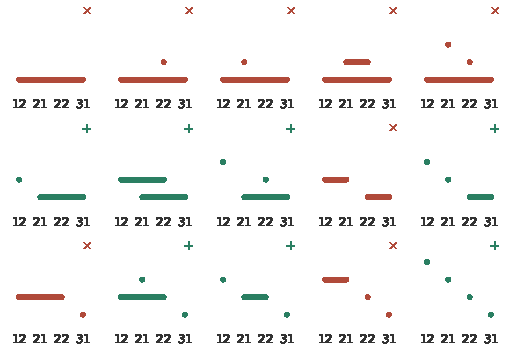
\includegraphics[width=0.98\linewidth]{figs_ws4/fig_census.pdf}
\caption{The census. Each panel draws one partition: a bar over a group
of states is a fibre (green when its common safe-action set is
nonempty, red when empty), and the margin marks adequacy
(\(+\)/\(\times\)). The two adequate two-cell partitions are panels 6
and 7 of the middle row.}
\label{fig:census}
\end{figure}

The maximal subsets with a nonempty common safe-action set are
\(\{(1,2), (2,2)\}\) and \(\{(2,1), (2,2), (3,1)\}\). They overlap in
\((2,2)\), so no partition into maximal common-action sets exists:
coarsening to maximal fibres is not an available design, and the
adequate partitions found by the census are the design options. The criterion is one-step
monitoring adequacy; dynamic viability is not claimed from it (the
kernels are computed by the full recursion). The census excludes
instrument \(0\) without loss: \(F_0 \le F_1\) and \(F_0 \le F_2\)
pointwise with the safe set an up-set (verified in the frame section)
give every one-step-safe fibre a safe instrument in \(\{1,2\}\). Two
consequences follow. Pairwise intersection of safe-action sets is necessary for fibre
adequacy; in the two-instrument audited universe it is also sufficient
(Helly number two: a pairwise-intersecting family of subsets of a
two-point action set has a common action), so every inadequate fibre in
the census fails with a literal empty intersection, while in action sets
of three or more elements pairwise intersection ceases to suffice
(\(\{1,2\}, \{2,3\}, \{1,3\}\)); and an
observation map merging states with disjoint safe-action sets obstructs
at that information state while every branch remains individually
viable --- the remedy is a fibre split, not a finer threshold on the
same index. The census makes both visible at the level of individual
fibres: in each inadequate partition of Table \ref{tab:census} the
failing fibre is exactly one merging \((1,2)\) --- whose safe-action
set is the singleton \(\{1\}\) --- with a state whose safe actions
exclude \(1\), i.e. \((2,1)\) or \((3,1)\), and each adequate
partition merges \((1,2)\) with neither. The census is itself an
instance of a structure:

\begin{proposition}[adequacy as an incompatibility-graph criterion]
\label{prop:adequacy}
Let \(G\) be the incompatibility graph of the target: vertices are
states, with an edge \((x, x')\) when \(R(x) \cap R(x') =
\emptyset\). A partition is adequate if and only if every fibre is an
independent set of \(G\); on the audited target the edges are exactly
\(\{(1,2)\text{--}(2,1),\ (1,2)\text{--}(3,1)\}\), so the adequate
partitions are the partitions into independent sets, counted by
inclusion--exclusion as \(15 - (5 + 5 - 2) = 7\) (the two edge events
overlap in exactly the \(2\) partitions whose fibre contains
\((1,2), (2,1), (3,1)\) jointly), and the adequate two-cell partitions
are exactly the graph's two proper \(2\)-colorings --- rows 6 and 7.
In an \(a\)-action universe, a fibre fails adequacy only through a
subfamily of at most \(a\) states with empty common intersection: the
Helly number of the family of subsets of an \(a\)-element action set
is \(a\) (verified exhaustively for \(a = 2\) and \(a = 3\), where the
minimal failing family \(\{\{1,2\}, \{2,3\}, \{1,3\}\}\) attains it);
pairwise intersection suffices only for \(a = 2\), and for convex
\(m\)-dimensional action domains the bound is \(m + 1\)
(Proposition~\ref{prop:helly}).
\end{proposition}

\begin{proof}
A fibre is adequate exactly when its states' safe-action sets intersect,
which is the complement of an edge exactly on two-state fibres and,
since the audited universe has Helly number two, for all fibres
(Proposition~\ref{prop:helly} is the \(m\)-dimensional analogue). The
edge count is the two disjointness facts above. The inclusion--exclusion
count: partitions whose fibres include the edge \((1,2)\text{--}(2,1)\)
are partitions of the three objects \(\{(1,2)(2,1)\}, (2,2), (3,1)\) ---
five; symmetrically five for the other edge; both edges force the
fibre \(\{(1,2), (2,1), (3,1)\}\) --- two partitions (with and without
\((2,2)\) merged). A two-cell adequate partition is a bipartition into
independent sets, i.e. a proper \(2\)-coloring of the star; there are
exactly two. The Helly statements are finite computations over all
subfamilies of the \(2^{a}\) subsets of an \(a\)-element set (exact for
\(a = 2, 3\); check P19).
\end{proof}

\subsection{Regime uncertainty}\label{regimes}

Two regimes alternate: an adversary chooses at the end of step
\(t - 1\) the regime realized at step \(t\). The model, explicit: the
controller acts one instrument \(u \in \{1,2\}\) per step (coordinate
\(u\) regenerates by one, cap \(3\)), and the acting regime deals one
unit of damage to its own coordinate (floor \(0\)); there is no other
change. With the regime frozen and announced, the controller drives the state
to a fixed point --- acting the damaged coordinate holds it wherever
its level is below the cap, and one step of the other instrument frees
a capped coordinate --- so the corner \((1,1)\) is
viable under each regime separately, and each frozen kernel comprises
all \(36\) belief pairs. Mode-blind operation, with the regime read
only through the state, yields a kernel of exactly 28 --- every pair
containing the corner is lost (from \((1,1)\) either instrument
regenerates one coordinate while the adversarial damage zeroes the
other), no merged-pair loss exists, and the loss is generated entirely
at the singleton level. The mode-blind kernel
agrees setwise with the full-information kernel of Section
\ref{classes}; the agreement is coincidental, arising under different
damage routings, and no identity is claimed. All three counts (frozen
\(36\) per regime, corner viable under each, mode-blind \(28\)) are
machine-verified from these primitives (check P13 of the verification script).

\subsection{The continuous benchmark}\label{benchmark}

A state is a pair of stocks \((x_1, x_2) \ge 0\) with a demand floor
on each; the aggregate is \(Y = x_1 + x_2\), and the \(Y\)-fibre is
the set of states with that aggregate. One control set
\(U = \{u \ge 0 : u_1 + u_2 \ge 2\}\) faces the floors through
Y-dependent caps \(\mathrm{cap}_1(Y) = 3/2 - (Y - 2)/10\) and
\(\mathrm{cap}_2(Y) = 59/50 - (Y - 2)/10\); an allocation \(u \in U\)
is feasible on the fibre when \(u_i \le \mathrm{cap}_i(Y)\) --- fibre
feasibility, not transition dynamics, is this section's audited object.
The critical aggregate is \(Y^{*} = 27/5\): the cap sum equals \(2\)
exactly there. Table
\ref{tab:bench} evaluates the caps on the audited aggregates and Figure
\ref{fig:bench} displays them. The \(Y = 5\) fibre is viable with
witness \((6/5, 4/5)\); the \(Y = 6\) fibre is obstructed with cap sum
\(47/25 < 2\), certified by the dual measure \((1/2, 1/2)\) on the two
active-floor atoms with margin \(3/50\). The crossover is again a general law:

\begin{proposition}[exact benchmark crossover]\label{prop:bench}
For every aggregate \(Y \ge 2\) with \(\mathrm{cap}_i(Y) \ge 0\), the
\(Y\)-fibre admits a feasible input (some \(u \in U\) with
\(u_i \le \mathrm{cap}_i(Y)\)) if and only if
\(\mathrm{cap}_1(Y) + \mathrm{cap}_2(Y) \ge 2\), which holds if and
only if \(Y \le 27/5\). For \(Y \ge 27/5\) the
\(\ell_1\)-normalized dual measure \((1/2, 1/2)\) on the two cap rows
certifies the obstruction with the exact margin
\(\tfrac12\bigl(2 - \mathrm{cap}_1(Y) - \mathrm{cap}_2(Y)\bigr) =
(Y - 27/5)/10\).
\end{proposition}

\begin{proof}
If the cap sum is at least \(2\), the input
\(u = (\mathrm{cap}_1(Y),\, 2 - \mathrm{cap}_1(Y))\) is nonnegative
(\(\mathrm{cap}_1(Y) \le 3/2 < 2\) on \(Y \ge 2\)), lies in
\(U\) (its coordinate sum is \(2\)), and respects the caps
(\(2 - \mathrm{cap}_1(Y) \le \mathrm{cap}_2(Y)\) is the cap-sum
inequality). Conversely any \(u \in U\) under the caps has
\(2 \le u_1 + u_2 \le \mathrm{cap}_1(Y) + \mathrm{cap}_2(Y)\), so a
cap sum below \(2\) is infeasible. The cap sum is the affine function
\(67/25 - (Y - 2)/5\), equal to \(2\) exactly at \(Y = 27/5\) and
declining beyond; the dual measure gives
\(\lambda^\top(\mathrm{cap} - u) = (\mathrm{cap\ sum})/2 -
(u_1 + u_2)/2 \le (\mathrm{cap\ sum})/2 - 1\), the stated margin.
\end{proof}

\begin{table}[t]
\centering
\footnotesize
\caption{The benchmark's cap arithmetic on the audited aggregates
(exact rationals). The cap sum crosses the demand level \(2\) exactly
at \(Y^{*} = 27/5\); at \(Y = 6\) the cap sum falls \(3/25\) short of
\(2\), and the \(\ell_1\)-normalized dual measure \((1/2, 1/2)\) certifies the
obstruction with margin \(3/50\).}
\label{tab:bench}
\begin{tabular}{@{}l c c c l@{}}
\toprule
\(Y\) & \(\mathrm{cap}_1\) & \(\mathrm{cap}_2\) & sum & reading\\
\midrule
4 & $13/10$ & $49/50$ & $57/25$ & above\\
$9/2$ & $5/4$ & $93/100$ & $109/50$ & above\\
5 & $6/5$ & $22/25$ & $52/25$ & viable (witness $(6/5, 4/5)$)\\
$27/5$ & $29/25$ & $21/25$ & $2$ & critical\\
$11/2$ & $23/20$ & $83/100$ & $99/50$ & below\\
6 & $11/10$ & $39/50$ & $47/25$ & obstructed, margin $3/50$\\
\bottomrule
\end{tabular}
\end{table}

\begin{figure}[t]
\centering
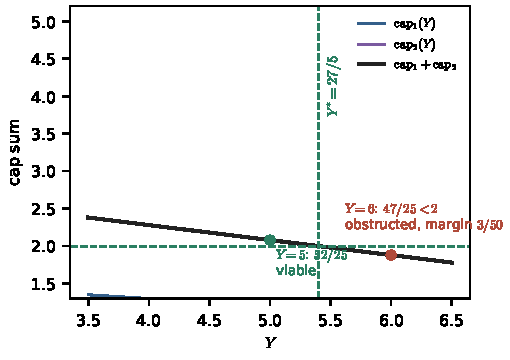
\includegraphics[width=0.96\linewidth]{figs_ws4/fig_benchmark.pdf}
\caption{The benchmark. Both caps decrease linearly in the aggregate
\(Y\); their sum crosses the demand level \(2\) exactly at
\(Y^{*} = 27/5\). The \(Y = 5\) fibre is viable (green), the \(Y = 6\)
fibre obstructed with margin \(3/50\) (red).}
\label{fig:bench}
\end{figure}

\subsection{Static duality}\label{duality}

Static duality for the benchmark's two floor rows, abstracted to drift
rows on \([0,1]\): the max--min equals the
min-\(\lambda\) max at value \(-1/10\), with multiplier
\(\lambda = (1/2, 1/2)\) the \(\ell_1\)-normalized Farkas pair of the calculus's
worked certificate (Abaee, 2026b). Figure \ref{fig:duality} displays
the instance: under the \(\ell_1\)-normalized multiplier the expected drift is
constant \(-1/10\) on all of \([0,1]\). Convexity is load-bearing: with
\(U = \{0, 1\}\) and rows \((-1, +1)\), \((+1, -1)\), the common set is
empty, the max--min is \(-1\), and the min-multiplier maximum is
\(0\). Under convexity the witness is sparse:

\begin{proposition}[static minimax duality on the two-floor instance]
\label{prop:saddle}
On the obstructed instance with drift rows \(\psi_1(u) = 2/5 - u\),
\(\psi_2(u) = u - 3/5\) on \(U = [0,1]\),
\[
\max_{u \in [0,1]} \min_i \psi_i(u) \;=\;
\min_{\lambda \in \Delta_2} \max_{u \in [0,1]}
\bigl(\lambda_1 \psi_1 + \lambda_2 \psi_2\bigr) \;=\; -\,\frac{1}{10},
\]
with the unique saddle point \((u^{*}, \lambda^{*}) = \bigl(1/2,
(1/2, 1/2)\bigr)\); under \(\lambda^{*}\) the expected drift is
constant \(-1/10\) on all of \([0,1]\).
\end{proposition}

\begin{proof}
The min envelope \(\min_i \psi_i(u)\) is concave and piecewise
linear with its peak at the crossing \(2/5 - u = u - 3/5\), i.e.\
\(u^{*} = 1/2\), value \(-1/10\). For \(\lambda \in \Delta_2\)
the pooled drift \((2\lambda_1 - 1)\cdot(-u) + \text{const}\) is
affine with slope \(\lambda_2 - \lambda_1 = 1 - 2\lambda_1\); it is
constant exactly at \(\lambda^{*} = (1/2, 1/2)\), where the value is
\(\tfrac12(2/5) + \tfrac12(-3/5) = -1/10\) for every \(u\). At any
other \(\lambda\) the maximum over \([0,1]\) is attained at an
endpoint; writing \(A(\lambda)\) for the \(u = 0\) endpoint value, the
two endpoint values are \(A(\lambda)\) and \(A(1 - \lambda)\), and
the averaging bound
\(\max(A(\lambda), A(1-\lambda)) \ge \tfrac12\bigl(A(\lambda) +
A(1-\lambda)\bigr) = -\tfrac1{10}\) --- the average is exactly the
constant value, for every \(\lambda\) --- with equality only at
\(\lambda^{*}\): the convexity of the max, not symmetry alone, locates
the minimum. Weak duality (max-min \(\le\) min-max)
holds unconditionally; the exhibited pair attains both sides at
\(-1/10\), which is therefore the exact common value and the unique
saddle.
\end{proof}

\begin{proposition}[sparse obstruction witnesses]\label{prop:helly}
An infeasible finite family of affine constraints on a convex domain in
\(\mathbb{R}^m\) has an infeasible subfamily of at most \(m + 1\)
members, and \(m + 1\) is tight. The instance realizes the bound: the
three constraints \(\{u_1 \ge 1,\ u_2 \ge 1,\ u_1 + u_2 \le 1\}\)
are pairwise feasible, jointly infeasible, and no two of them certify
the obstruction.
\end{proposition}

\begin{proof}
Intersect each constraint's halfspace with the domain: an infeasible
family of compact convex sets in \(\mathbb{R}^m\) has an infeasible
subfamily of size at most \(m + 1\) (Helly's theorem), and \(m + 1\)
is tight: the reversed halfspaces \(\{u_i \ge 1\}\) and
\(\sum_i u_i \le 1\) in \(\mathbb{R}^m\) --- the facets of an
\(m\)-simplex, translated outward --- meet \(m\) at a time and never
all \(m+1\) (the facets themselves meet in the simplex, which is why
the reversal is needed). For the
instance, each pair is feasible --- at \((1,1)\), \((1,0)\), and
\((0,1)\) respectively --- while all three give the contradiction
\(2 \le 1\); the verification script verifies each pair at its printed
feasible point and the triple by the exact contradiction.
\end{proof}

The Helly-tight family of three constraints
\(\{u_1 \ge 1,\ u_2 \ge 1,\ u_1 + u_2 \le 1\}\) --- no two of them
already infeasible --- attains the obstruction with \(m{+}1 = 3\)
constraints. The feasible contrast at rows
\((2/5 - u,\ u - 1/5)\) carries value \(+1/10\) on both sides of the
saddle: a certificate exists exactly where the value is negative, and at
a zero value the instance is boundary-critical with no strictly positive
margin available.
Weak duality (max--min \(\le\) min--max) holds unconditionally. Strong duality holds where its hypotheses are verified: the control set compact \emph{and convex}, the rows affine (or concave) in \(u\), and the label family finite --- as in the static instance above and the finite-horizon static-observation classes of the calculus (Abaee, 2026b). Both hypotheses are load-bearing: the paper's own nonconvex example (\(U = \{0,1\}\), rows \((-1,+1)\), \((+1,-1)\)) is compact, finite, and row-affine, yet gaps (\(-1\) against \(0\)); and continuity of the rows does not repair convexity, as the nonconvex rows example above shows --- concavity of the rows in \(u\), not continuity, is what the minimax argument consumes.

\begin{figure}[t]
\centering
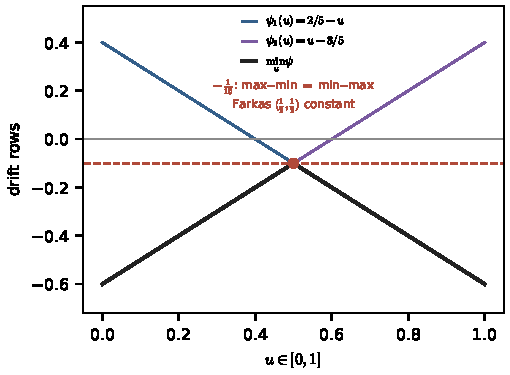
\includegraphics[width=0.96\linewidth]{figs_ws4/fig_duality.pdf}
\caption{Static duality on the two-floor instance. The two drift rows
cross at \(u = 1/2\); the max--min equals the min-multiplier maximum at
\(-1/10\), and the \(\ell_1\)-normalized Farkas pair \((1/2, 1/2)\) makes the
expected drift constant at the value.}
\label{fig:duality}
\end{figure}

\subsection{The certainty-equivalence drift audit}\label{drift}

For the index \(g(s) = s^{2}\) the uncorrected law's one-step drift is
\(g(s + 1/10) - g(s) = s/5 + 1/100\) on \([1,2]\): increasing, with
minimum \(21/100\) at \(s = 1\) and maximum \(41/100\) at \(s = 2\)
(Table \ref{tab:drift}); the corrected law's drift is identically zero --- by
construction, the corrected law being the lead removed. A biased
observation map misreads the state by a fixed one-step lead; on any
decision model conditioned on the map, that misreading is the mechanism
through which a nonempty kernel could empty, and the drift audit bounds
it exactly --- the remedy is structural correction of the map, not a
better sensor.

\begin{table}[t]
\centering
\footnotesize
\caption{The certainty-equivalence drift audit:
\(g(s + 1/10) - g(s) = s/5 + 1/100\) exactly; the corrected law's
drift is \(0\) at every probed state.}
\label{tab:drift}
\begin{tabular}{@{}l c c c@{}}
\toprule
\(s\) & uncorrected & corrected & increment per \(1/4\)\\
\midrule
1 & $21/100$ & 0 & \\
$5/4$ & $26/100$ & 0 & $1/20$\\
$3/2$ & $31/100$ & 0 & $1/20$\\
$7/4$ & $36/100$ & 0 & $1/20$\\
2 & $41/100$ & 0 & $1/20$\\
\bottomrule
\end{tabular}
\end{table}

\subsection{Multiple floors}\label{floors}

With several binding floors the Farkas certificate obstructs jointly: a
single certificate over all floors certifies nonviability where
per-floor certificates do not compose. On the audited benchmark's two
floors (Section \ref{benchmark}), the minimal infeasible subsystem
carries explicit witnesses --- the Helly-tight triple of Section
\ref{duality} --- and the corner \((1,1)\) is dynamically nonviable
as in the shared system. \emph{Quantifier and dual form.} Joint maintenance of several floors is the quantifier \(\exists u\ \forall j \in I(x)\) --- one control satisfying every active floor --- not \(\forall j\ \exists u_j\); per-floor certificates do not compose. The gap is visible in dimension one: on \(U = [-1, 1]\) the floors \(g_1(u) = u - \tfrac12 \ge 0\) and \(g_2(u) = -u - \tfrac12 \ge 0\) are each separately maintainable, yet no common control maintains both, and the \(\ell_1\)-normalized multiplier \(\lambda = (\tfrac12, \tfrac12)\) certifies the joint infeasibility with \(\sup_{u \in U}(\lambda_1 g_1 + \lambda_2 g_2)(u) = -\tfrac12 < 0\) --- a strict-separation dual certificate of exactly the Proposition~\ref{prop:helly} shape, with \(m + 1 = 2\) constraints necessary in dimension \(m = 1\) (each single floor is feasible). Scalar aggregation inherits the gap: a positive weighted average \(\sum_j \lambda_j h_j\) can conceal a violated component, and a multiplier inequality \(\sum_j \lambda_j \mathrm{D}h_j \ge 0\) does not imply that every active drift is nonnegative; the \(\ell_1\)-normalized dual measure of Section \ref{benchmark} certifies the aggregate shortfall exactly because both cap rows are charged jointly. In the audited convex static examples, infeasibility is certified by a multiplier supported on at most \(m + 1\) active constraints; no such bound is claimed for nonconvex controls or dynamic-policy images. Two further objects are recorded for subsequent study: a
first-breach timing bound for multi-floor systems, and a corner-cone
reading of the infeasibility region.

\subsection{Robustness margins}\label{margins}

Each certificate carries a margin, and each margin is a robustness
radius --- the size of the perturbation the certificate's verdict
tolerates.

\begin{proposition}[margins as radii]\label{prop:margins}
(i) \emph{Benchmark}: at \(Y = 6\) the obstruction survives any
per-cap increase \(\delta < 3/50\) of both caps and only there: the
certificate's margin \(3/50\) is exactly the per-cap robustness radius
(feasibility returns at \(\delta = 3/50\)). (ii) \emph{Timing}: the
boundary cells have zero slack (\(z_0 - 1 - T_{\mathrm{obs}} = 0\)):
any adversarial damage above unit rate flips them --- the inclusive
convention is exactly the statement that the audited identity holds on
zero-margin cells. (iii) \emph{Drift}: the corrected law's zero drift
has the sign of the correction error \(\varepsilon\) (\(2\varepsilon +
\varepsilon^2 = \varepsilon(2 + \varepsilon)\) at \(s = 1\)): the
sign-certificate is robust for every \(\varepsilon \in (-2, 0) \cup
(0, \infty)\). (iv) \emph{Decentralization}: each of the four forced
votes of the audited belief is knife-edge --- flipping that single vote
sustains nothing (zero margin, exact); the protocol's value is carried
by four coordinates, each of which is load-bearing.
\end{proposition}

\begin{proof}
(i) feasibility at \(Y = 6\) under uniform increases \(\delta\) is
\(\tfrac{47}{25} + 2\delta \ge 2 \iff \delta \ge
\tfrac{3}{50}\) --- exact arithmetic, checked at \(\delta =
\tfrac{3}{200}\) (infeasible) and \(\delta = \tfrac{3}{50}\)
(feasible). (ii) at \((z_0, T) = (2, 1)\) the worst damage under rate
\(1 + \varepsilon\) is \(1 + \varepsilon > 1 = z_0 - 1\). (iii) the
sign evaluation is the displayed factorization. (iv) for each forced
cell, the count of sustaining law pairs with that vote flipped is zero
(exhaustive over the \(256\) pairs; check P22).
\end{proof}

\subsection{Design rules}\label{rules}

The rules hold on the audited systems --- each an exact census identity or a proved general law, tagged by its evidence --- and transfer as default guidance only at that evidence level. \emph{Timing:} (proved general law, Proposition \ref{prop:timing}) reviews are boundary-inclusive ---
\(T_{\mathrm{obs}} \le \tau^{*}(z_0)\), the deadline at worst-case exit admissible under the audited endpoint convention (Section \ref{timing}). \emph{Coarseness:} (exact census, Section \ref{adequacy}) a fibre
merging states with disjoint safe-action sets obstructs at that
information state; the remedy is a fibre split, not a finer threshold
on the same index (Section \ref{adequacy}). \emph{Aggregation:} (exact census, Sections \ref{classes} and \ref{adequacy}) the aggregate index's fibres cross the safe boundary --- each mixes states of conflicting verdict --- and the aggregate kernel (\(26\) against the full \(28\)) certifies only a certainly-safe inner approximation; the certainly-safe set is the sound report.
\emph{Bias:} (exact audit, Section \ref{drift}) the uncorrected law's drift is at least \(21/100\) on a
101-point grid of \([1,2]\), while the corrected law's drift is
identically zero; a fixed bias is exactly correctable, and the remedy is
structural correction of the map, not a better sensor. The decentralized audit adds a final rule: (proved --- the restricted kernel is zero, Proposition \ref{prop:authority}) a whole-law authority restriction on one agent's vote collapses the sustainable set outright, so protocol
design precedes instrument tuning (Section \ref{decentralized}).

\subsection{Verification methods}\label{methods}

Every count, witness, identity, bound, figure, and tabulated entry in
this paper is regenerated by deterministic scripts in exact integer and
rational arithmetic, standard library only. The master verification
script recomputes the counts of Sections \ref{master}--\ref{regimes}
from the shared system's primitives --- the transition, the fibre
partition function, and the backward recursion with the no-repeat
protocol threaded as a parameter --- re-derives every tabulated entry of
Tables \ref{tab:master}, \ref{tab:laws}, \ref{tab:timing},
\ref{tab:census}, \ref{tab:bench}, and \ref{tab:drift} independently,
enumerates the census of Section \ref{adequacy}, evaluates the
benchmark identities of Section \ref{benchmark} in rational
arithmetic, asserts the drift bounds, and checks that each headline
number appears in the text. The figure-and-table generation script
recomputes and asserts each plotted or printed quantity from the same
primitives before drawing; the two scripts agree on every shared
quantity. The audited identities are additionally covered by the
per-system verification scripts of the companion papers (Abaee, 2026b;
see the Code availability statement). Two independent recomputation
paths guard the central recursions (checks P17--P18): an exhaustive
enumeration of all deterministic stationary policies --- \(2^{5} = 32\)
aggregate, \(2^{9} = 512\) full-information --- whose union of
safe-pair sets reproduces the kernels exactly (memoryless determinacy
on the instance, itself an exact verified fact), and a fixpoint
computation of each class's horizon family, whose stabilization equals
the audited kernel setwise. The recursion's cost is measured exactly:
the memoized backward recursion over the \(36\)-pair population uses
the distinct-subproblem counts printed by the script (states \(\times\)
horizon \(\times\) register per class), the policy enumerations use
\(32\) and \(512\) candidates, the decentralized census \(256\) law
pairs (\(64\) behavioral), the adequacy census \(15\) partitions, and
the two timing grids \(93\) cells each.

\subsection{Conclusion}\label{conclusion}

Exact audits bind the obstruction calculus to its worked systems: each
mechanism acquires a count, a witness, and a boundary. The timing
certificate fires everywhere beyond \(z_0 - 1\) and nowhere at the
boundary; the adequate monitoring designs on the audited target are
enumerable, and no coarsest one exists; policy-class value drops
unequally across aggregation and protocol restrictions, with the two
middle cells incomparable, the meet of their kernels institutional
setwise, and exactly one pair --- the alternation-forced pair --- beyond
both; unanimity costs a fixed and identified set of beliefs, sustained
by exactly the \(4 \times 4\) product of free votes, recoverable only
while both votes remain free; regime blindness loses exactly the
corner's pairs, while no frozen regime loses any; and the continuous
benchmark separates the viable from
the obstructed at \(Y^{*} = 27/5\) with rational certificates on both
sides. The incomparability of the middle cells is a shared-register
phenomenon: with per-branch registers the protocol cost collapses
(Proposition~\ref{prop:register}), which is precisely why the shared
register is the audited institutional object. The design rules --- boundary-inclusive reviews, fibre splits
over threshold tuning, certainly-safe reporting under aggregation,
structural repair of bias, and protocol design before instrument tuning
--- are the audit's operational content, and the master table is its
evidence: every count in the paper is one column of one table, every entry of which is regenerated by script. These examples do not constitute a general taxonomy of viability failures; they supply exact counterexamples, finite censuses, and reproducible benchmarks that separate mechanisms often conflated in qualitative discussion. Read through the master theorem, the audit is a small theory: the five mechanisms --- common-action failure, memory/register coupling, finite-time boundary exit, decentralized information loss, and joint convex infeasibility --- each carry a certificate, a monotonicity status under the theorem's three axes, a requirement-level characterization (statewise factoring for unanimity, incompatibility-graph adequacy for fibres, max-plus hitting times for regimes), and a robustness radius (\(3/50\) per cap on the benchmark, zero on the boundary cells and the forced votes, sign-robustness on the drift)

\subsection*{References}

Abaee, A., 2026a. Robust viability of the 2J3KL limit reference point
under a surplus-production map: policy scoring, expansion, and when
catch cannot help. Zenodo.
\url{https://doi.org/10.5281/zenodo.22552060}

Abaee, A., 2026b. An obstruction calculus for viability under
incomplete observation (submitted).

\subsection*{Declarations}

\subsection*{Funding}
None.

\subsection*{Competing interests}
None.

\subsection*{Data availability}
No external data were used.

\subsection*{Code availability}
The verification script \url{paper2_worked_systems_v13_verification.py}
and the figure-and-table generation script
\url{paper2_worked_systems_figures.py} are publicly available at
\url{https://github.com/MIKEAA2020/general-sustainability} (folder
\texttt{arena agent 1/paper rewrites/latex}); they reproduce all
counts, witnesses, bounds, figures, and tabulated entries verbatim.

\subsection*{AI declaration}
GLM (Z.ai), Qwen (Alibaba Cloud) and DeepSeek AI assisted with drafting
and iterative review. The author reviewed and edited outputs and takes
responsibility for the final work.

\end{document}
